\chapter{Results}

In this section are presented the main outcomes obtained when simulating the wind turbine model described preivously.  First are presented the results estimated for a wind turbine rotor that is is alligned with the incoming flow. Next are presented the same results but for a rotor that it is not laterally alligned with the incoming flow, named as yawed rotor. After that its is described the effect of some extra features included in the BEM analysis such as the influence of the tip correction and numerical discretization, the evaluation of stagnation enthalpy or the evaluation of the system's circulation and vorticity.\\

Describe the initial conditions, table, cool


\section{BEM alligned rotor}

In this section it is considered that the rotor is fully alligned with the incoming flow as it would be in an ideal case. The discretization used to compute the main results includes 50 divisions in the radial position. The discretization is uniformly spaced using the same increment between adjacent sections.  

\subsection{Main outputs }

The main outputs described in this sections would help the user identify the behaviour of the key variables that affect the rotor performance. Under this conditions the variables will only see its values affected by the radial position and not by their azimuthal position. The results are easily represented using only one value (the weighted average) per span section in a 2D plot that represents the variable versus the span section.  

\subsubsection{\textbf{Angle of attack and inflow angle}  \textcolor{red}{BERNAT}}

In Fig. \ref{Inflow_alligned} are displayed the inflow angle and angle of attack of each tip speed ratio study case. 

\begin{figure}[htbp]
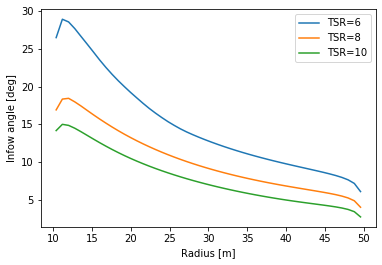
\includegraphics[width=0.75\textwidth]{./img/Inflow_plt_alligned.png}
\caption{Inflow angle vs. Radius distribution at different TSR values}
\centering
\label{Inflow_alligned}
\end{figure}

\begin{figure}[htbp]
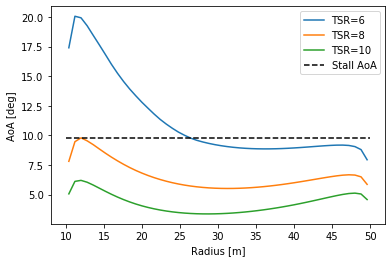
\includegraphics[width=0.75\textwidth]{./img/AoA_plt_alligned.png}
\caption{Angle of attack vs. Radius distribution at different TSR values}
\centering
\label{AoA_alligned}
\end{figure}

The results are coherent with the tip speed ratio defiinition. In the study the freeflow incoming velocity is fixed at 10 m/s, so for the different TSR values the parameter changing is the rotor rotational speed $\Omega $. At higher $\Omega $ values the rotational speed component is bigger and thus the inflow angle will decrease as shown in the plots. The angle of attack distribution also matches. Per definition, the geometrical twist of the blade could be obtained from these plots as the difference between the inflow angle and the angle of attack, which is a function of the $\mu$ parameter. \\

It must be higlighted that for the TSR=6 the inboard part of the blade is under stall conditions, hence will be a poor power generation section. This can be concluded because the stall AoA is included in the plot. In this study the stall AoA has a contstant value along the entire span because the blade is built entirely with the same airfoil model. In commercial WTGs the blades use different airfoils depending on the radial section. If this WT model had to be design to operate most of the time under these conditions the optimal aerodynamic performance would probably be given at a TSR between 6 and 8. Because as it can be seen from Fig XXX , the maximum CL/CD ratio is obatined at AoA ranged between 7.5 and 9.25 degrees.

\begin{figure}[htbp]
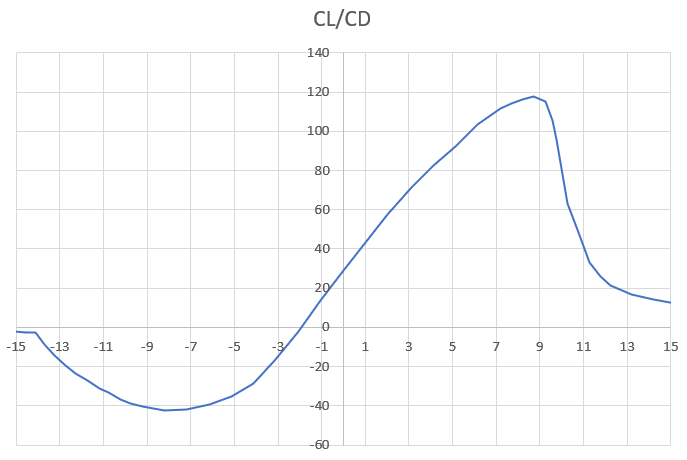
\includegraphics[width=0.75\textwidth]{./img/CL_CD_plt.png}
\caption{CL/CD ratio vs. Radius }
\centering
\label{CL_CD_alligned}
\end{figure}


\subsubsection{\textbf{Axial and azimuthal inductions}  \textcolor{red}{BERNAT}}

In Fig. \ref{Inflow_alligned} are displayed the distribution of axial and tangential inductions of TSR case study. 

\begin{figure}[htbp]
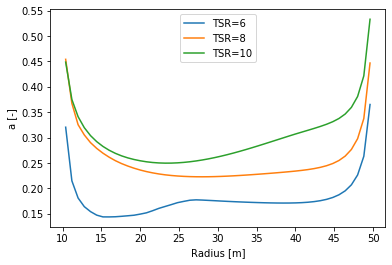
\includegraphics[width=0.75\textwidth]{./img/a_plt_alligned.png}
\caption{Axial induction factor vs. Radius distribution at different TSR values}
\centering
\label{a_alligned}
\end{figure}

\begin{figure}[htbp]
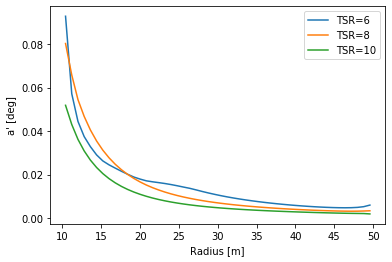
\includegraphics[width=0.75\textwidth]{./img/ap_plt_alligned.png}
\caption{Tangential induction factor vs. Radius distribution at different TSR values}
\centering
\label{ap_alligned}
\end{figure}



\subsubsection{\textbf{Thrust and azimuthal loading} \textcolor{red}{BERNAT}}

In Fig. \ref{thrust_alligned} are displayed the distribution of axial and tangential loads acting on the rotor for each TSR case study. 

\begin{figure}[htbp]
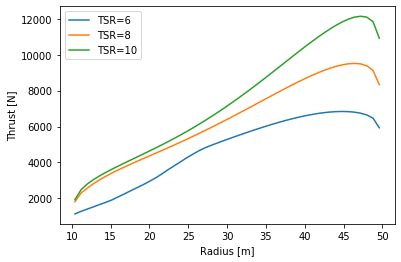
\includegraphics[width=0.75\textwidth]{./img/thrust_plt_alligned.png}
\caption{Thrust vs. Radius distribution at different TSR values}
\centering
\label{thrust_alligned}
\end{figure}

\begin{figure}[htbp]
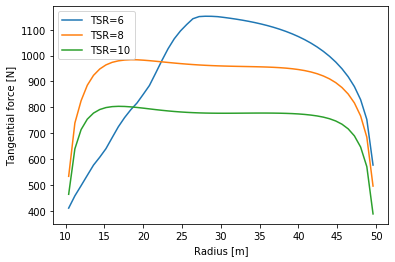
\includegraphics[width=0.75\textwidth]{./img/tang_plt_alligned.png}
\caption{Tangential force vs. Radius distribution at different TSR values}
\centering
\label{tang_alligned}
\end{figure}

As it is mentioned in the previous subsection, in the TSR=6 operation regime the inboard part of the blade (approximately until 25m) loses its capacity to extract energy from the wind to generate thrust and torque. Under these conditions the inboard sections are experiencing inflow and AOA angles too high and the cross-sections airfoils are operating outside their optimal regime. This effect could have been partly mitigated if the polars of those inner sections would have been corrected by the 3D effects such as the Snel correction proposed in the introduction. \\

The most intensively-loaded sections are the ones closer to the tip. This was expected by looking at the AoA radial distribution. Those sections operate at the uppper range of the CL lienar region, close to stall, where the CL/CD ratio is better. But the AoA is not the only parameter afecting the performance, if it was like that the curves at higher TSR would generate larger loads. It has to be taken into account that in the way the TSR modifications in this assignment consider the incoming flow velocity $U_{\infty}$ and Blade Radius $R$ constant, meaning that the only paraeter changing its value is the rotor speed $\Omega$. Thus, what is being done when increasing the TSR is increasing the absolute value of the relative velocity seen by the sections, which would end up increasing severly the loads as it afects the term that is at a power of 2. 

\subsubsection{\textbf{Total thrust and torque} \textcolor{red}{BERNAT}}

Table \ref{total_forces_alligned} provides the values obtained for the total Thrust and Torque generated by the WTG at the different TSR. The total thrust force hass been computed as the sum of the axial forces $fx$ generated by each annulus section. The total torque has been computed as the sum of the products of the tangential force $fy$ and the radial position $r$ of each annular section. In the previous sections the loads have been provided without taking into account the density, thus with units $ \frac{N}{Kg/m^3} $. However, in Table XXX the total forces have been estimated for a standard density $\rho = 1.225 kg/m^3$ to give a better overview of the rotor performance.

\begin{table}[htpb]
\begin{tabular}{lllll}
\cline{2-4}
\multicolumn{1}{l|}{}                            & \multicolumn{1}{l|}{\textbf{TSR = 6}} & \multicolumn{1}{l|}{\textbf{TSR = 8}} & \multicolumn{1}{l|}{\textbf{TSR = 10}} &  \\ \cline{1-4}
\multicolumn{1}{|l|}{\textbf{Thrust {[}kN{]}}}   & \multicolumn{1}{l|}{235.443}          & \multicolumn{1}{l|}{316.605}          & \multicolumn{1}{l|}{369.669}           &  \\ \cline{1-4}
\multicolumn{1}{|l|}{\textbf{Torque {[}kN�m{]}}} & \multicolumn{1}{l|}{1464.494}         & \multicolumn{1}{l|}{1361.402}         & \multicolumn{1}{l|}{1116.159}          &  \\ \cline{1-4}
\end{tabular}
\label{total_forces_alligned}
\end{table}


\section{BEM yawed rotor \textcolor{blue}{NIKLAS}}

The results in this section were obtained for the rotor operating with tip speeds $\lambda = 6,8,10$ and yaw values of $\psi = 15, 30$ degrees. The discretization used here is the same as in section 3.1, however, since for the yawed case variables are not constant over the azimuth the discretization also includes 4 equally spaced divisions over the azimuth. 

\subsection{Main outputs \textcolor{blue}{NIKLAS}}
The main outputs in this section would help the user identify how the key variables that affect rotor performance are changed by a yaw angle of the incoming flow. The variables will vary radially and azimuthally and are, unless otherwise specified, averaged over the azimuth to give 2D plots that show variation only over the span.

\subsubsection{\textbf{Angle of attack and inflow angle} \textcolor{blue}{NIKLAS}}
\begin{figure}[htbp]
	\centering
	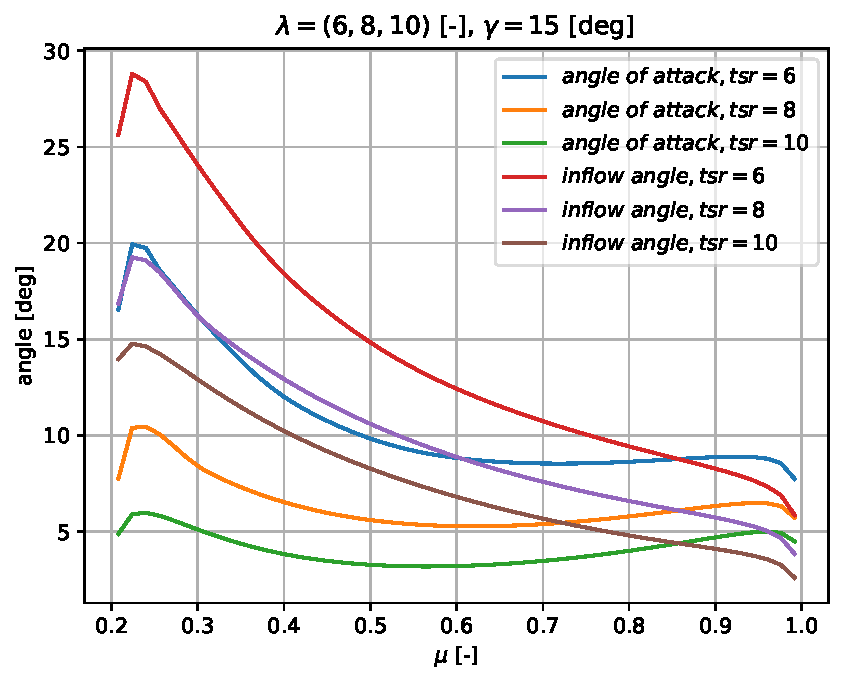
\includegraphics[height=0.45\textheight]{./img/yaw/alpha_phi-yaw_15.pdf}
	\caption{Angle of attack and inflow angle at a yaw of 15 degrees.}
	\label{img:yaw-aoa-15}
\end{figure}
\begin{figure}[htbp]
	\centering
	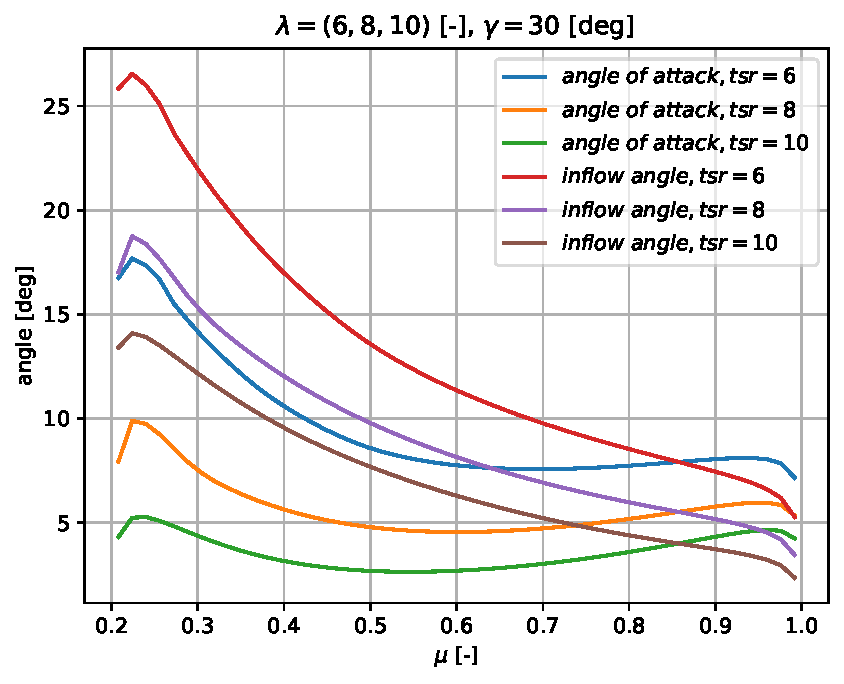
\includegraphics[height=0.45\textheight]{./img/yaw/alpha_phi-yaw_30.pdf}
	\caption{Angle of attack and inflow angle at a yaw of 30 degrees.}
	\label{img:yaw-aoa-30}
\end{figure}
Figures \ref{img:yaw-aoa-15} and \ref{img:yaw-aoa-15} show the spanwise distribution of the angle of attack and inflow angle for TSR = 6,8,10 and for yaw angles of 15 and 30 degrees respectively. These plots are very similar in shape to the non-yawed case with the inflow angle decreasing with increasing radial direction and TSR. Since increasing TSR means increasing rotational speed the inflow angle decreases due to a larger rotational speed component. Similarly, since the rotational speed increases with increasing radial position the inflow angle also decreases closer to the tip of the blade.
It is again apparent that for TSR=6 the inboard part of the blade is under stall conditions. It should also be noted that for increasing yaw angles both the angle of attack and the inflow angle decreased for all TSR. This means that for a higher yaw angle and TSR=6 less of the blade is under stall conditions.

\subsubsection{\textbf{Axial and azimuthal inductions} \textcolor{blue}{NIKLAS}}
\begin{figure}[htbp]
	\centering
	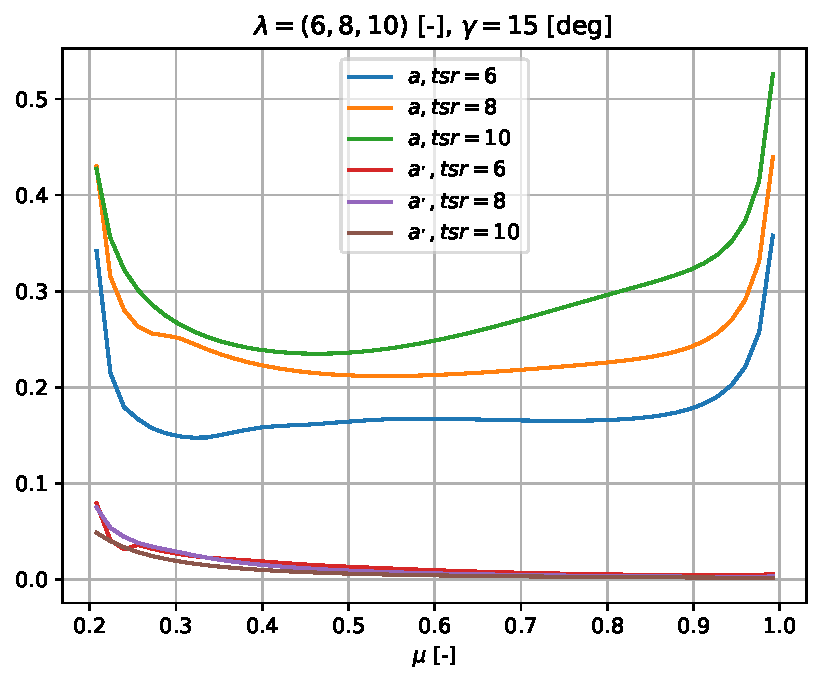
\includegraphics[height=0.45\textheight]{./img/yaw/a_aip-yaw_15.pdf}
	\caption{Axial and azimuthal inductions at yaw of 15 degrees.}
	\label{img:yaw-aap-15}
\end{figure}
\begin{figure}[htbp]
	\centering
	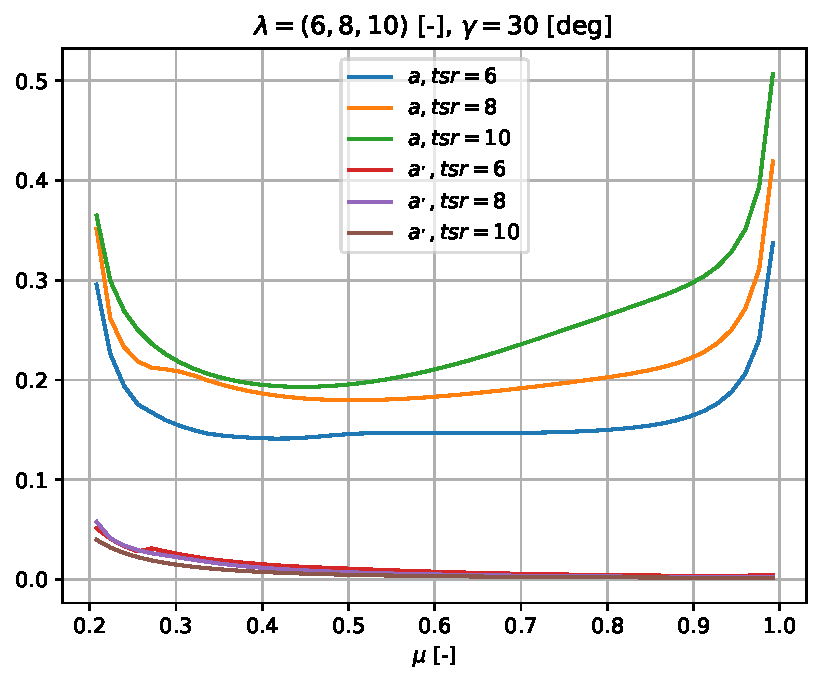
\includegraphics[height=0.45\textheight]{./img/yaw/a_aip-yaw_30.pdf}
	\caption{Axial and azimuthal inductions at yaw of 30 degrees.}
	\label{img:yaw-aap-30}
\end{figure}
Figures \ref{img:yaw-aap-15} and \ref{img:yaw-aap-30} present the spanwise distribution of the axial and azimuthal inductions, $a$ and $a^,$. The shape of these plots is similar to the non-yawed case, however, the values for both axial and azimuthal inductions decrease with increasing yaw angle.

\subsubsection{\textbf{Thrust and azimuthal loading} \textcolor{blue}{NIKLAS}}
\begin{figure}[htbp]
	\centering
	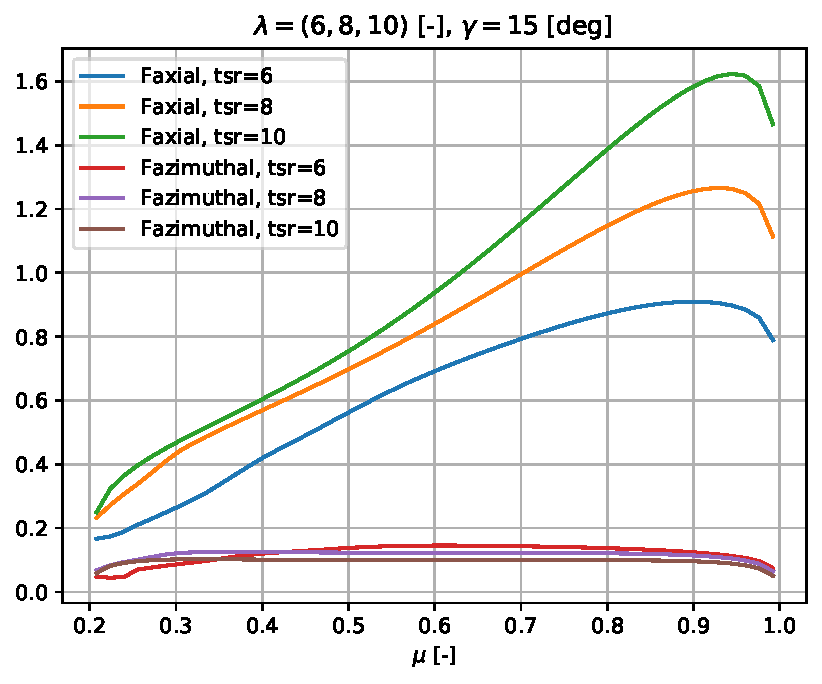
\includegraphics[height=0.45\textheight]{./img/yaw/Fax_Faz-yaw_15.pdf}
	\caption{Thrust and azimuthal loading normalized by $\frac{1}{2} \rho U_\infty^2 R$.}
	\label{img:yaw-f-15}
\end{figure}
\begin{figure}[htbp]
	\centering
	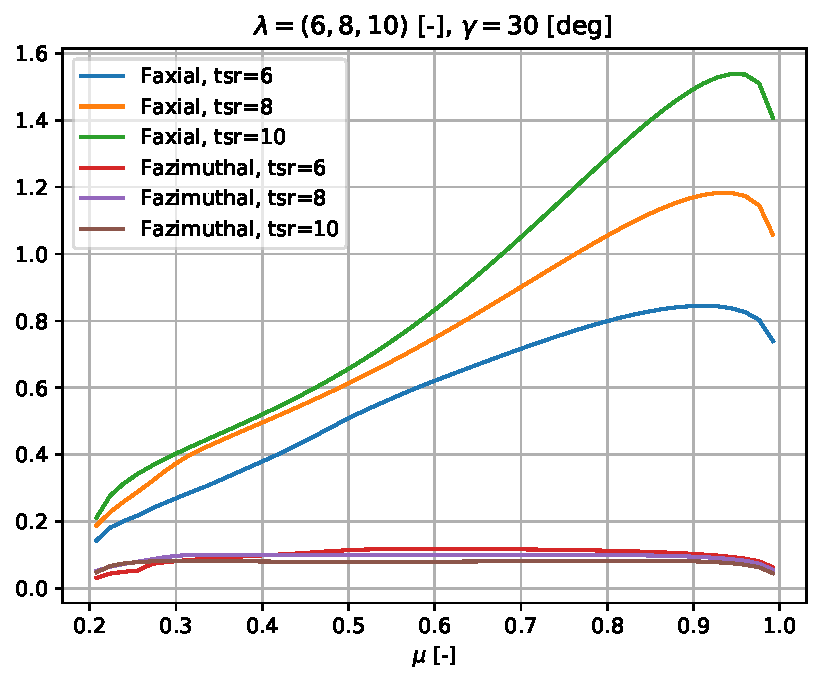
\includegraphics[height=0.45\textheight]{./img/yaw/Fax_Faz-yaw_30.pdf}
	\caption{Thrust and azimuthal loading normalized by $\frac{1}{2} \rho U_\infty^2 R$.}
	\label{img:yaw-f-30}
\end{figure}
Figures \ref{img:yaw-f-15} and \ref{img:yaw-f-30} present the spanwise distribution of the thrust and azimuthal loading on the blade. The shape of the plots again mirrors the non-yawed case except that the values decrease with increasing yaw. Note that the axial thrust increases with increasing TSR, while the azimuthal loading decreases with increasing TSR. It should also be noted that for TSR=6 the azimuthal loading near the root drops off. This is because for TSR=6 the blade near the root is under stall conditions.

\subsubsection{\textbf{Total thrust and torque} \textcolor{blue}{NIKLAS}}
Tables \ref{tbl:thrust-15} and \ref{tbl:thrust-30} provide the values of the total thrust and torque generated by the wind turbine at TSR=6,8,10 and yaw angles 15 and 30 degrees respectivly. The total thrust was computed by taking the average axial force over the azimuth of each annulus section and taking their sum. Similartly, the total torque was computed by taking the average tangential force over the azimuth of each annulus section and taking their sum. As in the non-yawed case these loads were calculated without density and so a standard density $\rho = 1.225 kg/m^3$ was used.
\begin{table}[h]
\caption{\textbf{Thrust and Torque for yaw angle of 15 degrees.}}
\begin{tabular}{|l|l|l|l|}
\hline
   & \textbf{TSR=6} & \textbf{TSR=8} & \textbf{TSR=10}  \\ \hline
\textbf{Thrust {[}kN{]}} &   230.370    &  305.932    &   359.225     \\ \hline
\textbf{Torque {[}kN*m{]}} &  1378.321   &  1273.163     &   1050.505     \\ \hline
\end{tabular}
\label{tbl:thrust-15}
\end{table}

\begin{table}[h]
\caption{\textbf{Thrust and Torque for yaw angle of 30 degrees.}}
\begin{tabular}{|l|l|l|l|}
\hline
   & \textbf{TSR=6} & \textbf{TSR=8} & \textbf{TSR=10}  \\ \hline
\textbf{Thrust {[}kN{]}} &   211.879    &  276.674     &   326.935     \\ \hline
\textbf{Torque {[}kN*m{]}} &   1137.425    &  1035.234     &   858.573     \\ \hline
\end{tabular}
\label{tbl:thrust-30}
\end{table}

\subsubsection{\textbf{Azimuthal Variation} \textcolor{blue}{NIKLAS}}
For the case of a yawed turbine the results are not constant over the azimuth. This variation is presented here in Fig. \ref{img:contour} for the axial induction for TSR=6 and a yaw of 15 degrees. The figure was computed using a discretization of 50 radial sections and 50 azimuthal sections. While there is some variation with the azimuth it is much less than the variation that occurs in the radial direction at the tip and root of the blades. This means that while the power extraced is reduced there are no significant extra loads on the blade to prevent operation. Thus it is sufficiant to analyze the values averaged over the azimuth.

\begin{figure}[htbp]
	\centering
	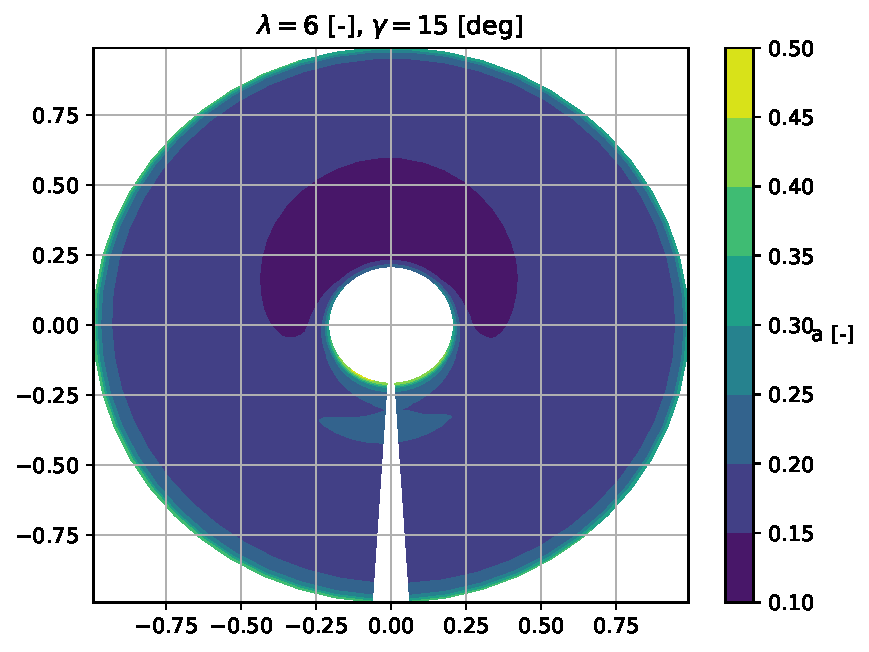
\includegraphics[height=0.45\textheight]{./img/yaw/contour-n_az-51.pdf}
	\caption{The azimuthal variaton of the axial induction.}
	\label{img:contour}
\end{figure}

\subsection{\textbf{Influence of numerical discretization} }

This subsection provides information about the influence that the numerical discretization has in the final results. The rotor conditions taken to carry out this analysis are at fixed at TSR = 8 and $U_{\infty} $ = 10 m/s. For the yawed cases the missalignment angle is set to 15 degrees. \\

The first analysis is focused on the effect of the different spacing methods to apply in the radial divisions. The most straight-forward is to use an uniformly spaced distribution that has a constant radius increment in adjacent sections. The proposed alternative in this study is to use a cosine-spaced radial distribution. This method is widely used for executing panel methods on 2D airfoils because an airfoil usually has more curvature on the LE. Hence, for more a more accurate calculation in this region it is necessary to have finer divisions. Figure XXX provides an example of how the distrubution of $\mu$ nodes will be for a 15-nodes configuration using the two methods mentioned. The values in the y-axis are irrelevant, are just separated enough to provide a good overview of the x-axis discretization. 

\begin{figure}[htbp]
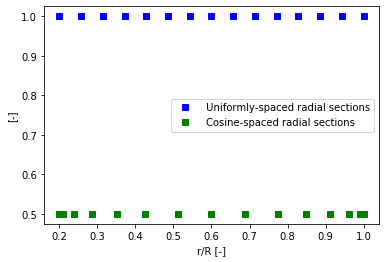
\includegraphics[width=0.75\textwidth]{./img/ex_cos_plt.png}
\caption{Distribution of 15 $\mu$ nodes with different division strategies }
\centering
\label{mu_nodes}
\end{figure}

Taking into account Figure XXX it can be seen that the cosine spaced distribution provides smaller divisions at the edges of the range. For the WT model this would mean that the more refined regions in the study are in the root and tip of the rotor. Both regions have the feature to be the ones where the Prandtl tip correction factor has more effect and where it is also varying more with respect to the span. This is the main reason why it has been decided to use this kind of discretization here. The results for both methodologies are ploted in Figure \ref{thrust_conv_alligned}. From this data it is obvious to conclude that the cosine spaced discretization is more efficient and converges faster. However it has to be mentioned that when forcing strict convergence tolerances the code has some trouble convergeing for more than 61 cosine-spaced divisions. This is probably due to the very tinny sections at the root and tip. Nevertheless, in the plot the value of Thrust for more than 61 divisions has been kept constant as it can be argumented that the 60th value was the exact value, as it keeps the asympthotic trend showed by the uniformly spaced cases. So to reach the converged value with the uniform distribution it will be necessary to use around 100 sections, while for the cosine it is enough with 50, only the half of it. Thus, using the cosine sapce could save up to 50$\%$ of the computational effort. 

\begin{figure}[htbp]
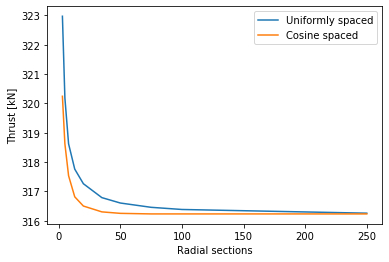
\includegraphics[width=0.75\textwidth]{./img/Thrust_convergence_plt.png}
\caption{Total Thrust convergence vs. number of radial sections}
\centering
\label{thrust_conv_alligned}
\end{figure}

Then a similar study has been carried out for the yawed case at 15 degrees and with 50 radial divisions for each method. Figure \ref{Thrust_conv_az_plt} displays the results obtained when using different numbers of azimutal sections. Again, this study has been executed for the two radially spaced methods. In this case it can bee seen that both methods do not converge in the same total Thrust value. This can be explained by looking again at Fig. \ref{thrust_conv_alligned}. From this plot it can be extracted that at 50 radial sections, both methodologies had not yet reached the same value. This is the difference seen in Fig. \ref{Thrust_conv_az_plt}. It is also worth to highlight that number of azimutal sections convergence seems to be decoupled of the radial discretization methdodology. Both techniques show variable behaviour until around 12 sections, where they reach a stable value. So computing the BEM in arcs of 30º seems to yield reliable results with this configuration.  


\begin{figure}[htbp]
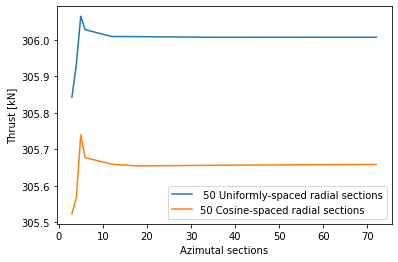
\includegraphics[width=0.75\textwidth]{./img/Thrust_conv_az_plt.png}
\caption{Total Thrust convergence vs. number of azimutal sections}
\centering
\label{Thrust_conv_az_plt}
\end{figure}



\section{Influence of the tip correction \textcolor{green}{CARLOS}}

The results shown in this section were obtained for the rotor described in the assignment instructions, operating with a tip speed ratio $ \lambda = 8 $ and no yaw. It can be seen that the tip correction reduces the power and thrust, resulting in a worse performance. Indeed, the rotor without the tip correction has a higher $ C_P/C_T $ ratio.

Near the blade tip, the flow angle $ \phi $ is reduced due to the tip vortex (Figure \ref{img:tc-phi}), because it induces a larger axial velocity (Figure \ref{img:tc-a}). Having a lower flow angle $ \phi $ results in a reduced power extraction, which is proportional to $ c_l \sin \phi - c_d \cos \phi $ (Figure \ref{img:tc-dcp-dmu}) \cite{weh-ch3}. However, reducing the flow angle $ \phi $ contributes to an increase of the thrust, since it is proportional to $ c_l \cos \phi + c_d \sin \phi $.

Note that $ c_l $ also decreases due to the reduction of $ \phi $, because it implies a decrease of the angle of attack $ \alpha $ (Figure \ref{img:tc-alpha}). Moreover, the relative velocity, which also affects the loads, will also be larger for the case without tip correction.

The tip correction tries to account for this effect. The expression Prandtl derived for that factor is shown in equation \ref{eq:f-prandtl}. Its value over the blade is plotted in Figure \ref{img:tc-f}. It relates the induction factor near the blade $ a_b $ with the azimuth average $ a $: $ a_b = a/f $ \cite{weh-ch3}.

\begin{equation}
f(\mu) = \frac{2}{\pi} \arccos \left[ \exp \left( - \frac{B}{2} \left( \frac{1-\mu}{\mu} \right) \sqrt{1+\frac{\lambda^2\mu^2}{(1-a)^2}} \right) \right]
\label{eq:f-prandtl}
\end{equation}

\begin{itemize}
	
	\item Power coefficient $ C_P $
	\begin{itemize}
		\item Tip correction: 0.4528
		\item No tip correction: 0.4757
		\item Increase: 5.05 \%
	\end{itemize}
	
	\item Thrust coefficient $ C_T $
	\begin{itemize}
		\item Tip correction: 0.6581
		\item No tip correction: 0.6691
		\item Increase: 1.67 \%
	\end{itemize}
	
	\item Power to thrust ratio $ C_P/C_T $
	\begin{itemize}
		\item Tip correction: 0.6880
		\item No tip correction: 0.7109
		\item Increase: 3.32 \%
	\end{itemize}
	
\end{itemize}

\begin{figure}[htbp]
	\centering
	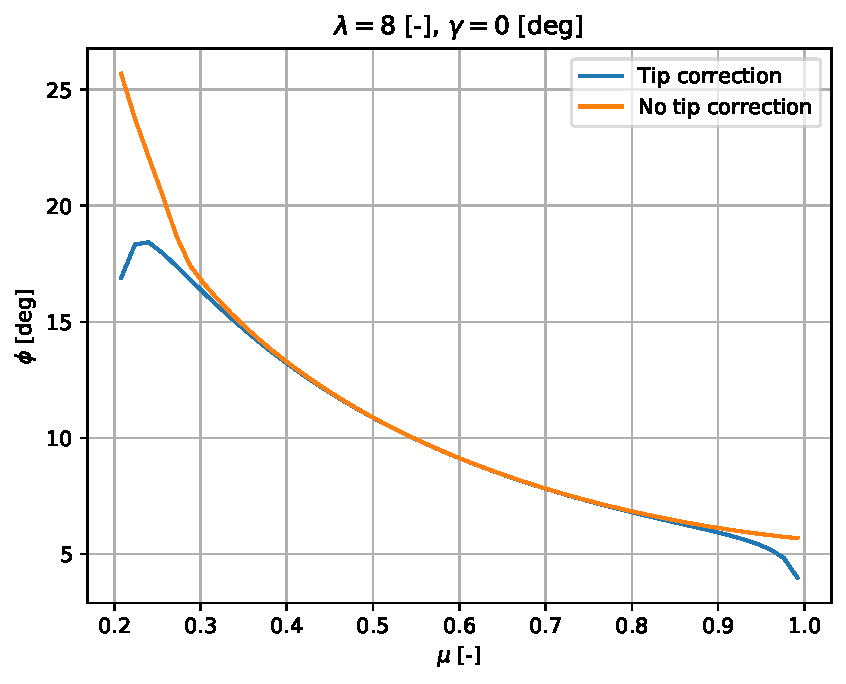
\includegraphics[height=0.45\textheight]{./img/tip-correction/phi.pdf}
	\caption{Flow angle distribution with and without tip correction.}
	\label{img:tc-phi}
\end{figure}

\begin{figure}[htbp]
	\centering
	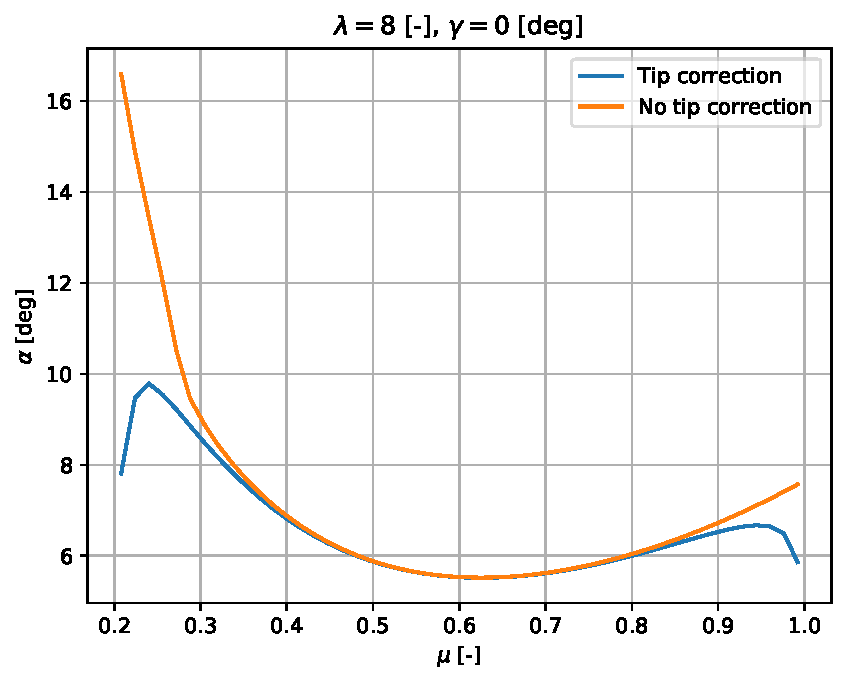
\includegraphics[height=0.45\textheight]{./img/tip-correction/alpha.pdf}
	\caption{Angle of attack distribution with and without tip correction.}
	\label{img:tc-alpha}
\end{figure}

\begin{figure}[htbp]
	\centering
	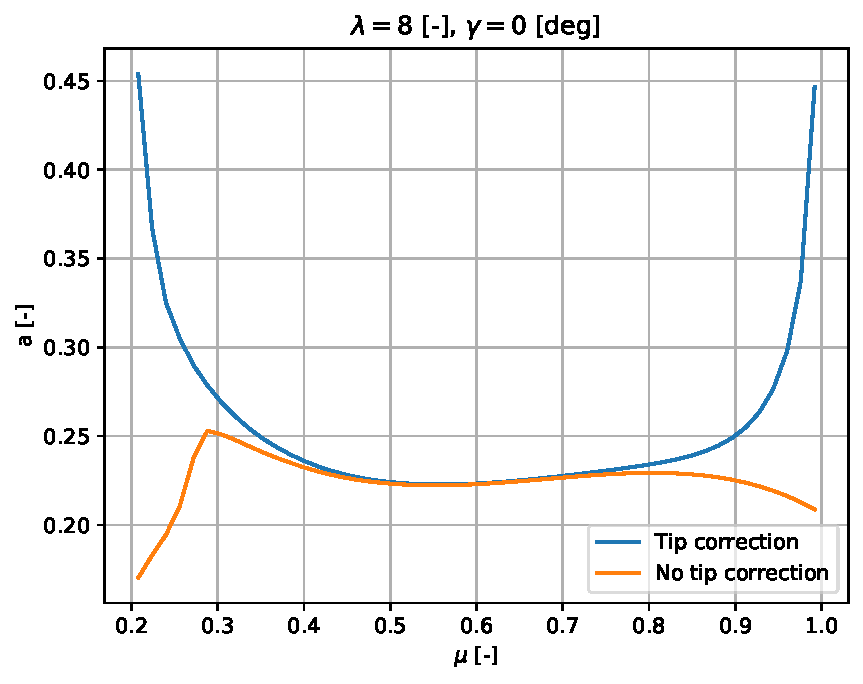
\includegraphics[height=0.45\textheight]{./img/tip-correction/a.pdf}
	\caption{Axial induction distribution with and without tip correction.}
	\label{img:tc-a}
\end{figure}

\begin{figure}[htbp]
	\centering
	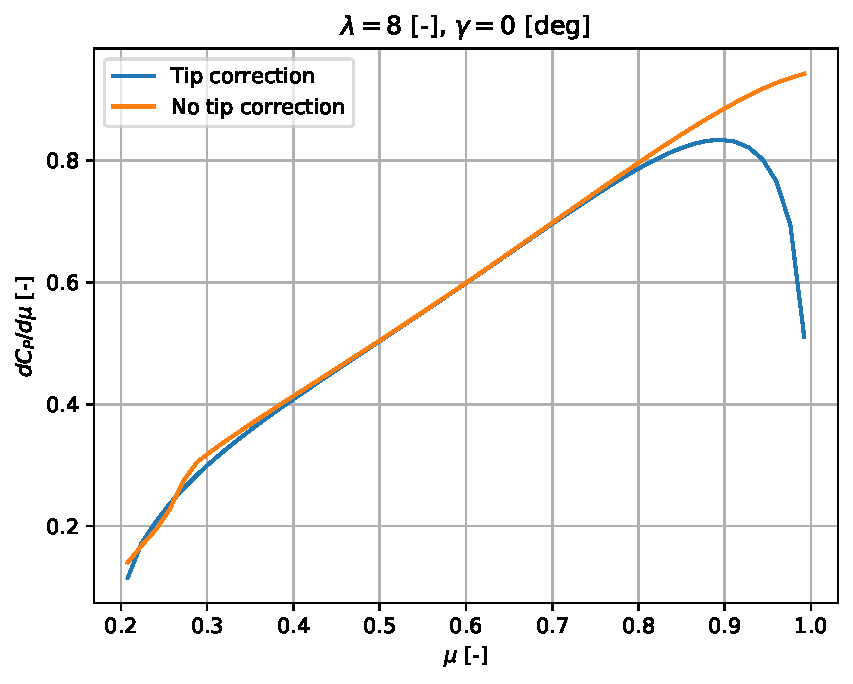
\includegraphics[height=0.45\textheight]{./img/tip-correction/dcp_dmu.pdf}
	\caption{Power coefficient distribution with and without tip correction.}
	\label{img:tc-dcp-dmu}
\end{figure}

\begin{figure}[htbp]
	\centering
	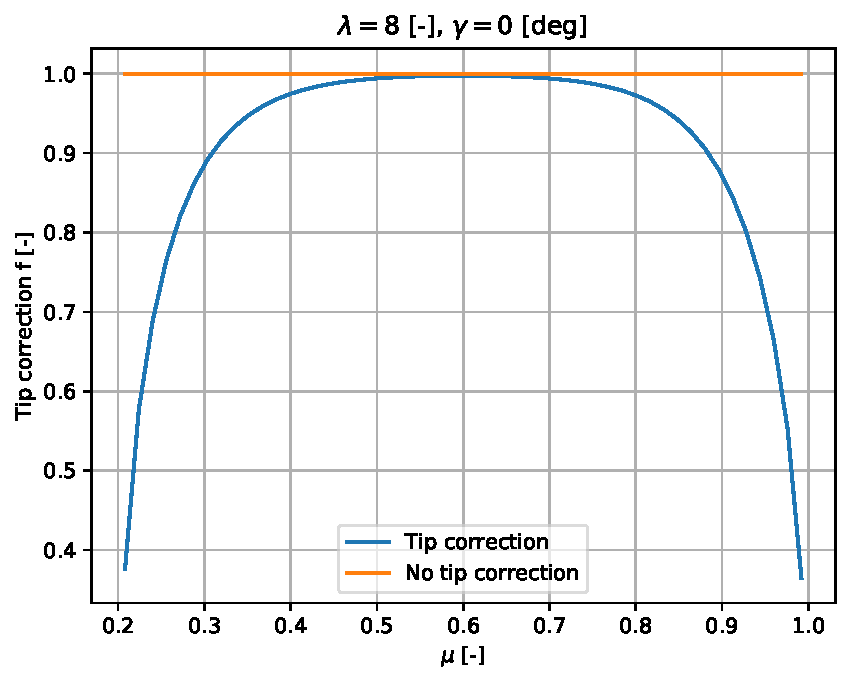
\includegraphics[height=0.45\textheight]{./img/tip-correction/f.pdf}
	\caption{Prandtl's tip loss factor distribution with and without tip correction.}
	\label{img:tc-f}
\end{figure}


\section{Evaluation of stagnation enthalpy \textcolor{green}{CARLOS}}

If heat exchange, viscous forces and compressibility effects are neglected, the flow temperature does not change. Therefore, it can be assumed that the air's internal energy is always constant. Then, the changes in stagnation enthalpy and stagnation pressure are equivalent. The mechanical energy equation (\ref{eq:mech-energy}) describes how the stagnation pressure $ p_t $ changes. Note that it has been obtained as the scalar product of the momentum equation and the velocity vector.

\begin{equation}
	\vec{v} \cdot \vec{\nabla} p_t = \vec{v} \cdot \vec{\nabla} \cdot \vec{\vec{\tau}} + \vec{v} \cdot \vec{f}
	\label{eq:mech-energy}
\end{equation}

If viscous forces are not considered, $ \tau = 0 $, the stagnation pressure can only due to the body forces $ b $ work. The only domain region where these forces are not null, and therefore, exert some work is the rotor plane. This means that the stagnation pressure only changes across the rotor plane. See equations (\ref{eq:pt-up}) and (\ref{eq:pt-down}) for the stagnation pressure expressions up and down-stream of the rotor plane respectively. They are plotted in Figure \ref{img:pt}.

\begin{equation}
	p_{t_u} = p_a + \frac{1}{2} \rho u_{\infty}^2
	\label{eq:pt-up}
\end{equation}

\begin{equation}
	p_{t_d} = p_a + \frac{1}{2} \rho u_{\infty}^2 (1-2a)^2
	\label{eq:pt-down}
\end{equation}

\begin{figure}[htbp]
	\centering
	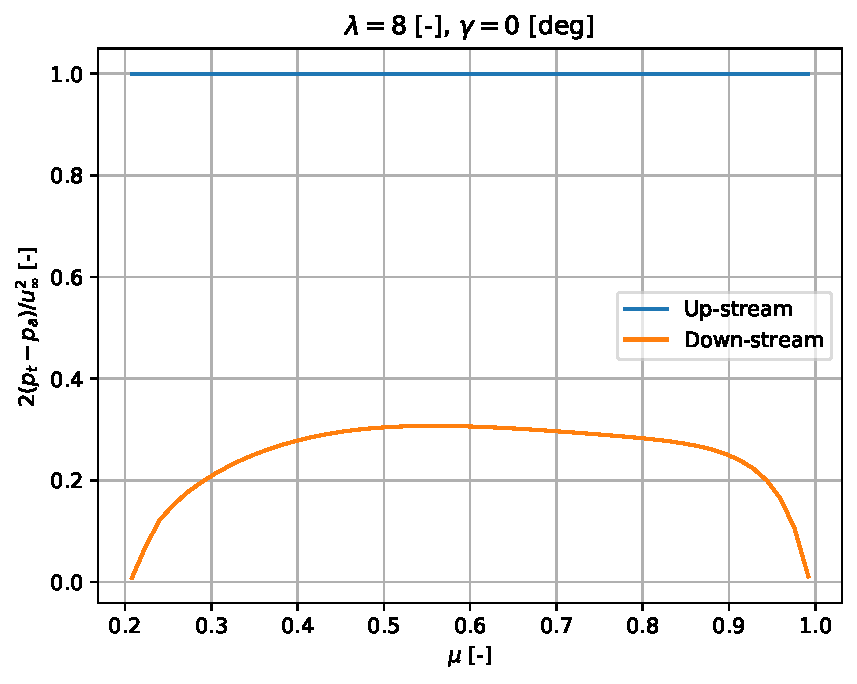
\includegraphics[height=0.45\textheight]{./img/stagnation-enthalpy.pdf}
	\caption{Stagnation enthalpy distribution.}
	\label{img:pt}
\end{figure}

\section{System of circulation and vorticity \textcolor{green}{CARLOS}}

The circulation distribution over the blade is shown in Figure \ref{img:gamma_}. It has a more or less constant shape in the centre part of the blade, and vanishes quite steeply near the root and tip. This seems reasonable, since circulation is related to lift generation by the Kutta-Joukowski theorem: $ l = \rho u_{\infty} \Gamma $. In the blade extremes, lift must be zero, since there is no surface that can create it.

\begin{figure}[htbp]
	\centering
	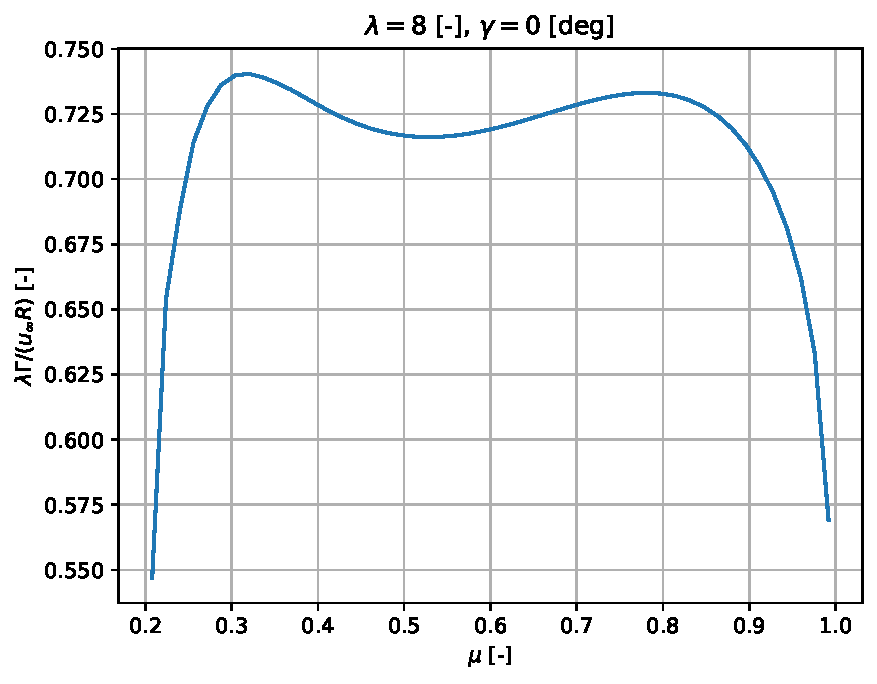
\includegraphics[height=0.45\textheight]{./img/circulation/gamma_.pdf}
	\caption{Circulation distribution.}
	\label{img:gamma_}
\end{figure}

The vorticity equation and Kutta-Jukowski theorem explain the changes observed in circulation. The thrust derivative with respect to the radius can be expressed using the Blade Element Theory, Kutta-Jukowski theorem and assuming no drag (\ref{eq:dT_dr_kj}), or using the Momentum Theory (\ref{eq:dT_dr_mt}).

\begin{equation}
	\frac{dT}{dr} = l \cos \phi = \rho w \Gamma \cos \phi
	\label{eq:dT_dr_kj}
\end{equation}

\begin{equation}
	\frac{dT}{dr} = \rho u_{\infty} (1-a) u_{\infty} 2a 2\pi r
	\label{eq:dT_dr_mt}
\end{equation}

If the expressions (\ref{eq:dT_dr_kj}) and (\ref{eq:dT_dr_mt}) are equated, it can be seen that the circulation is related to the local thrust. This is shown in Figure \ref{img:vort-forces}, where the two sides of equation (\ref{eq:gamma-ct}) are plotted. The slightly higher values for the thrust coefficient may be due to the drag contribution, which is not accounted for in the circulation.

\begin{equation}
	\frac{w \Gamma \cos \phi}{u_{\infty}^2 \pi r} = 4a(1-a) = C_T
	\label{eq:gamma-ct}
\end{equation}

\begin{figure}[htbp]
	\centering
	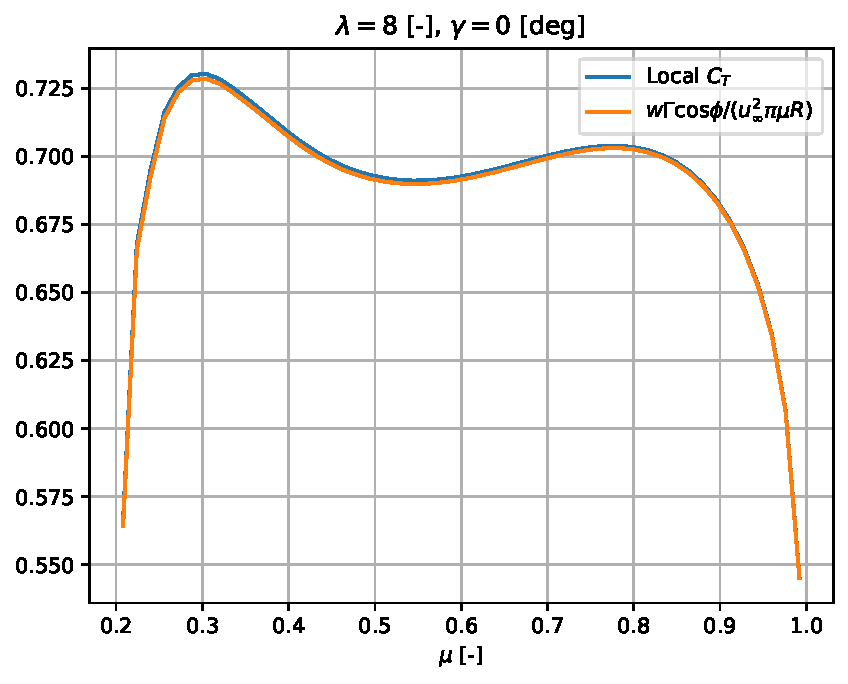
\includegraphics[height=0.45\textheight]{./img/circulation/vort-forces.pdf}
	\caption{Circulation and local thrust coefficient distribution.}
	\label{img:vort-forces}
\end{figure}

Equation (\ref{eq:gamma-ct}) is actually a different form of the vorticity equation (\ref{eq:vorticity}).

\begin{equation}
	\vec{v} \cdot \vec{\nabla} \vec{\omega} = \vec{\nabla} \times \vec{f}
	\label{eq:vorticity}
\end{equation}

Assuming there are no radial forces, and that vorticity only changes in its direction ($d\omega_i/dx_j = 0$, if $ i \neq j $), the vorticity equation in the tangential direction can be simplified to better show how it relates to expression (\ref{eq:gamma-ct}).

\begin{equation}
	w \cos \pi \frac{d\omega}{rd\theta} = - \frac{df_x}{dr}
	\label{eq:vort-tang}
\end{equation}

If equation (\ref{eq:vort-tang}) is integrated over the volume, expression \ref{eq:gamma-ct} is obtained. Remark that $ \int 1/r d\omega/d\theta dV = - \int \omega dS = - \Gamma $, and $ \int df_x/dr dV = dT/dr $.

The same procedure can be done for the vorticity generation in the axial direction. In this case, the vorticity equation is the one shown in (\ref{eq:vort-axial}). The relationship between the circulation and tangential force is given by equation (\ref{eq:gamma-cs}).

\begin{equation}
	w \sin \pi \frac{d\omega}{dx} = \frac{df_{\theta}}{dr}
	\label{eq:vort-axial}
\end{equation}

\begin{equation}
	\frac{dS}{dr} = l \sin \phi = \rho w \sin \phi \Gamma = \rho u_{\infty} (1-a) \Omega r 2a' 2 \pi r
	\label{eq:gamma-cs}
\end{equation}

The relationship between the tangential force and generation of circulation in the axial direction is depicted in Figure \ref{img:vort-forces-ax}. The differences observed may be due to the drag, which reduces the tangential force created by the lift.

\begin{figure}[htbp]
	\centering
	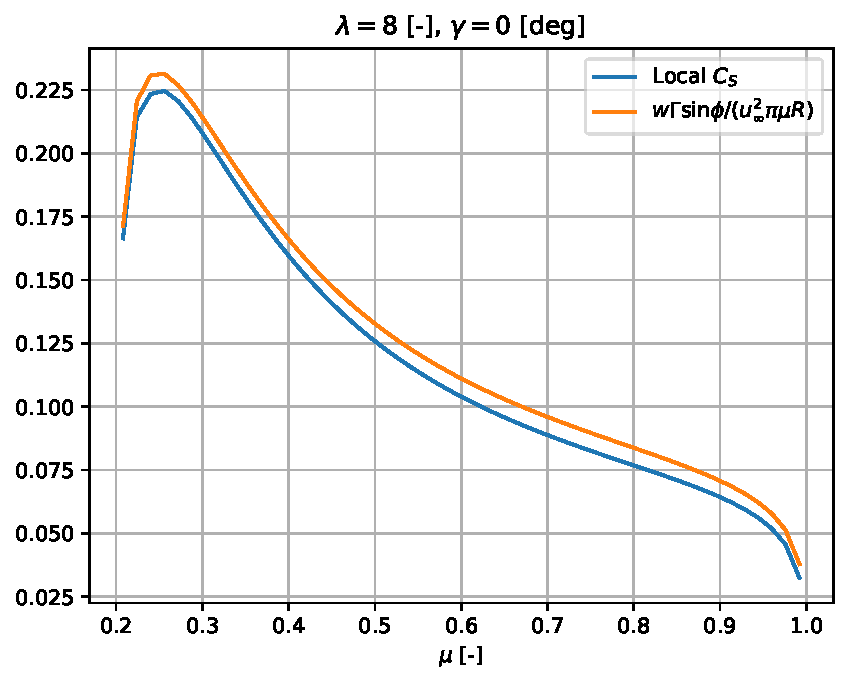
\includegraphics[height=0.45\textheight]{./img/circulation/vort-forces-ax.pdf}
	\caption{Circulation and local tangential coefficient distribution.}
	\label{img:vort-forces-ax}
\end{figure}

\section{Operational point \textcolor{blue}{NIKLAS}}
In this study the blades of the rotor used only one airfoil, the DU 95-W-180. The lift and drag polars of this airfoil were provided. 

\begin{figure}[htbp]
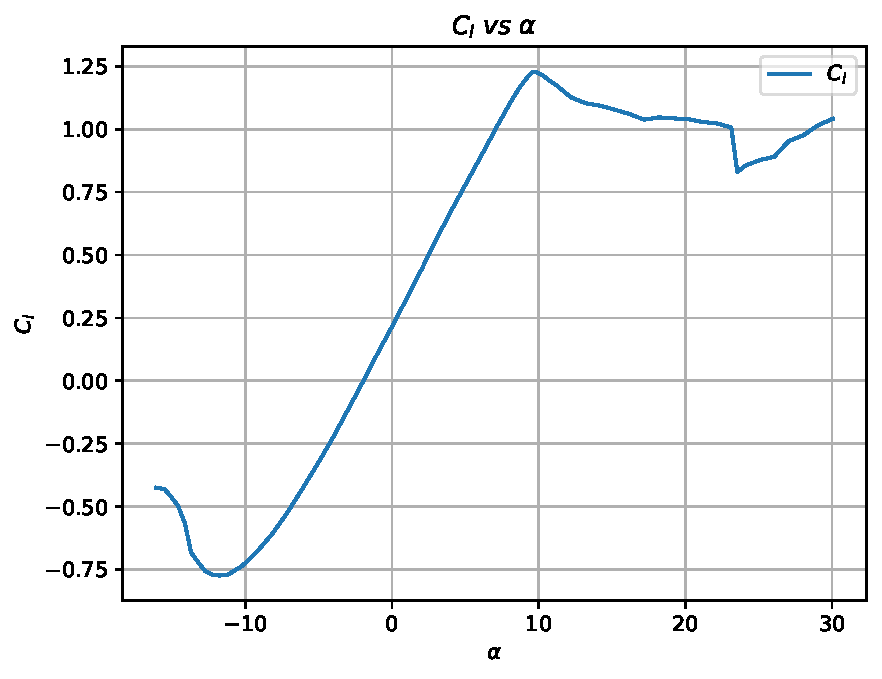
\includegraphics[width=0.75\textwidth]{./img/yaw/Cl_v_alpha.pdf}
\caption{$C_l\ v\ \alpha$ for the DU 95-W-180 airfoil.}
\centering
\label{img:clva}
\end{figure}
\begin{figure}[htbp]
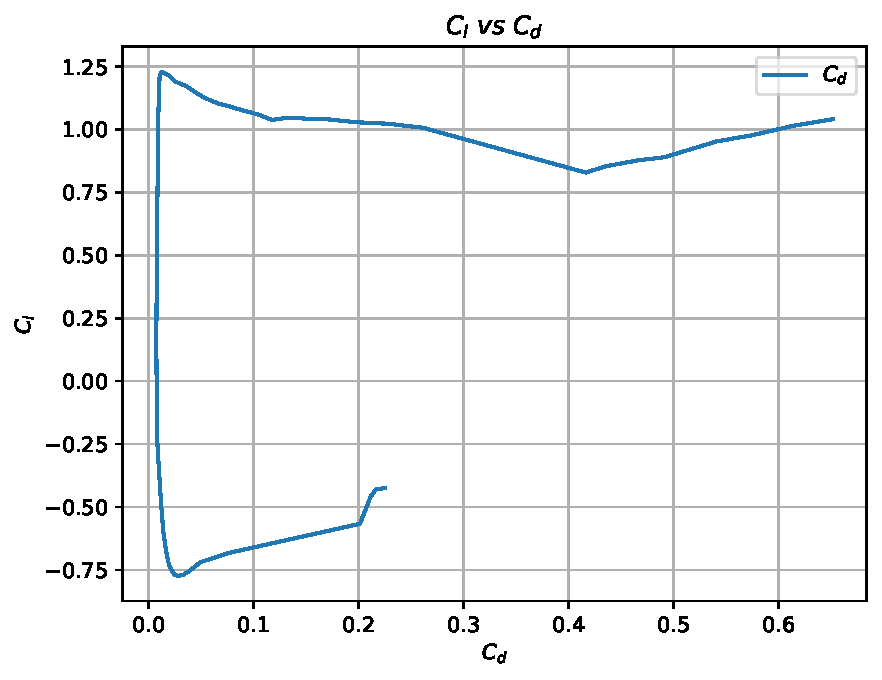
\includegraphics[width=0.75\textwidth]{./img/yaw/Cd_v_Cl.pdf}
\caption{$C_l\ v\ C_d$ for the DU 95-W-180 airfoil.}
\centering
\label{img:clvcd}
\end{figure}



